\chapter{Kết quả và thảo luận}

\section{Kết quả khảo sát OFAT đối với hệ Ag@PVP}
Kết quả khảo sát đơn yếu tố đối với hệ Ag@PVP được trình bày theo trình tự tỷ lệ glycerol, nồng độ NaOH, nhiệt độ phản ứng, thời gian phản ứng và nồng độ PVP.
Đối với từng khảo sát, các yếu tố không được thay đổi được giữ cố định theo điều kiện đã lựa chọn ở bước khảo sát trước đó.
Phổ UV--Vis được sử dụng để theo dõi sự xuất hiện, vị trí và cường độ của dải hấp thụ SPR.

\subsection{Khảo sát ảnh hưởng của tỷ lệ glycerol}
Hình~\ref{fig:pvp-glycerol} trình bày phổ UV--Vis của hệ Ag@PVP khi tỷ lệ glycerol được khảo sát tại 30, 40, 50, 60 và 70\% (v/v).
Sự thay đổi vị trí, cường độ và độ rộng của dải SPR được sử dụng để đánh giá ảnh hưởng của tỷ lệ glycerol đến quá trình hình thành AgNPs.

\begin{figure}[htbp]
  \centering
  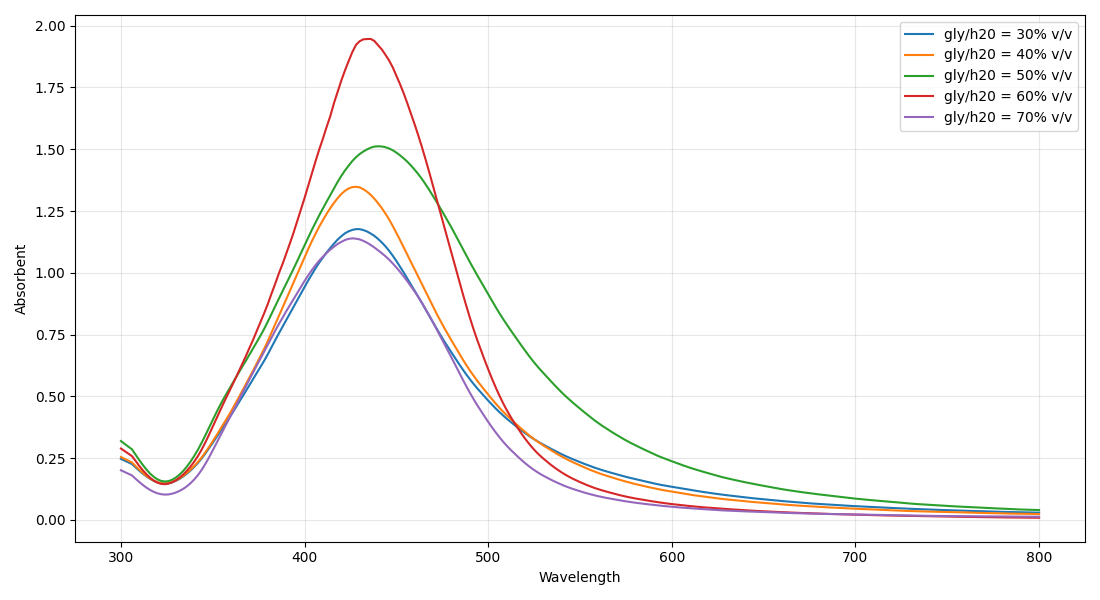
\includegraphics[width=0.95\textwidth]{figures/pvp_gly.png}
  \caption{Phổ UV--Vis của hệ Ag@PVP tại các tỷ lệ glycerol 30, 40, 50, 60 và 70\% (v/v).}
  \label{fig:pvp-glycerol}
\end{figure}

\subsection{Khảo sát ảnh hưởng của nồng độ NaOH}
Hình~\ref{fig:pvp-naoh} trình bày phổ UV--Vis của hệ Ag@PVP tại các nồng độ NaOH 0; 1,0; 1,5; 2,0; 2,5 và 3,0 mM.
Kết quả được sử dụng để đánh giá vai trò của điều kiện kiềm đối với sự hình thành và đặc trưng quang học của AgNPs.

\begin{figure}[htbp]
  \centering
  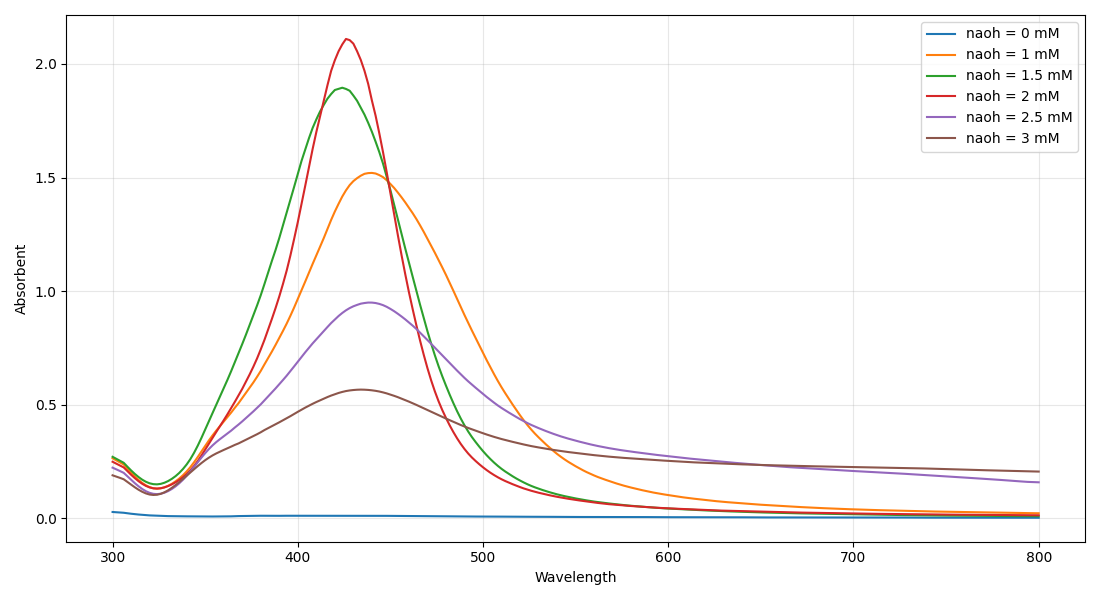
\includegraphics[width=0.95\textwidth]{figures/pvp_naoh.png}
  \caption{Phổ UV--Vis của hệ Ag@PVP tại các nồng độ NaOH 0; 1,0; 1,5; 2,0; 2,5 và 3,0 mM.}
  \label{fig:pvp-naoh}
\end{figure}

\subsection{Khảo sát ảnh hưởng của nhiệt độ phản ứng}
Hình~\ref{fig:pvp-temperature} trình bày phổ UV--Vis của hệ Ag@PVP khi nhiệt độ phản ứng được khảo sát tại 40, 50, 60, 70 và 80~$^\circ$C.
Sự thay đổi dải SPR theo nhiệt độ được xem xét cùng với các tiêu chí lựa chọn điều kiện phù hợp của hệ.

\begin{figure}[htbp]
  \centering
  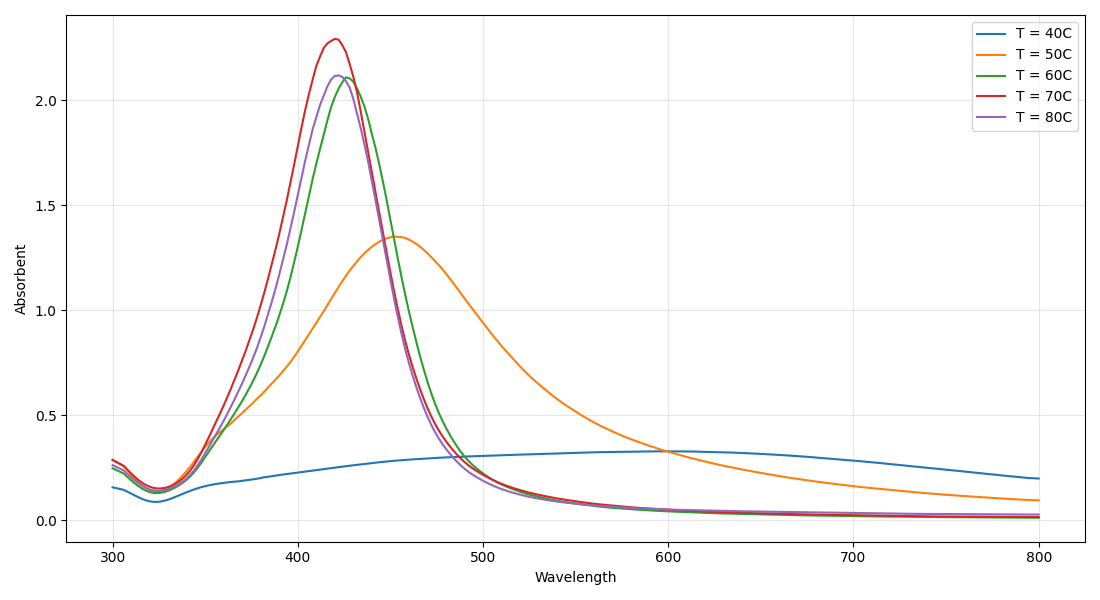
\includegraphics[width=0.95\textwidth]{figures/pvp_temp.png}
  \caption{Phổ UV--Vis của hệ Ag@PVP tại các nhiệt độ phản ứng 40, 50, 60, 70 và 80~$^\circ$C.}
  \label{fig:pvp-temperature}
\end{figure}

\subsection{Khảo sát ảnh hưởng của thời gian phản ứng}
Hình~\ref{fig:pvp-time} trình bày phổ UV--Vis của hệ Ag@PVP tại các thời điểm 5, 10, 15, 20, 25, 30 và 35 phút.
Các phổ được sử dụng để theo dõi diễn biến hình thành AgNPs theo thời gian phản ứng.

\begin{figure}[htbp]
  \centering
  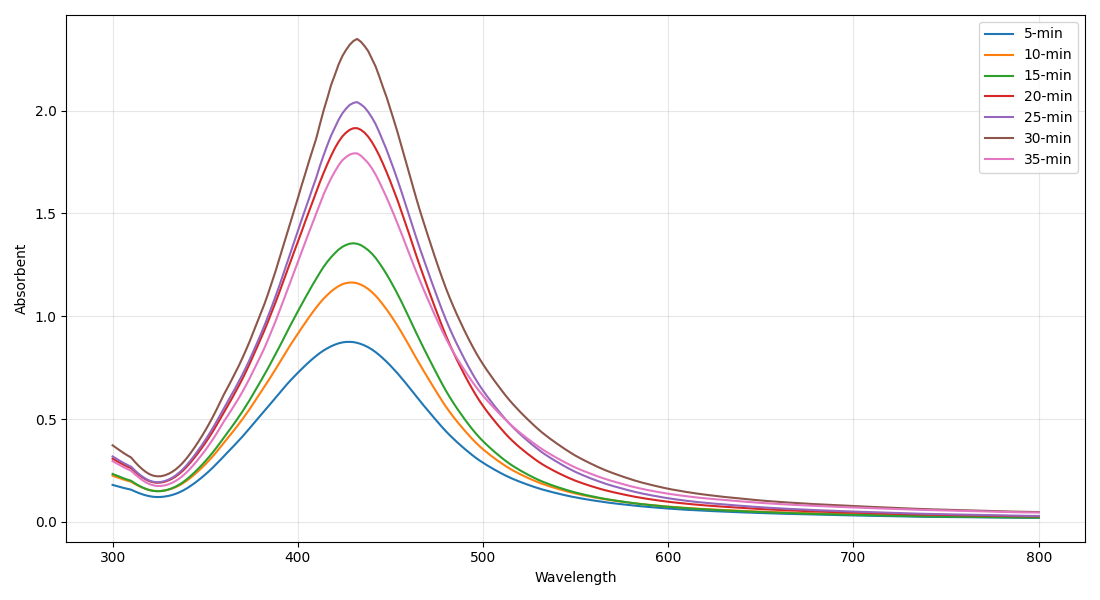
\includegraphics[width=0.95\textwidth]{figures/pvp_time.png}
  \caption{Phổ UV--Vis của hệ Ag@PVP tại các thời gian phản ứng 5, 10, 15, 20, 25, 30 và 35 phút.}
  \label{fig:pvp-time}
\end{figure}

\subsection{Khảo sát ảnh hưởng của nồng độ PVP}
Hình~\ref{fig:pvp-concentration} trình bày phổ UV--Vis của hệ Ag@PVP khi nồng độ PVP được khảo sát tại 0; 1; 2; 3 và 4\% (w/v).
Mẫu không bổ sung PVP được sử dụng làm đối chứng để đánh giá vai trò của polymer bảo vệ đối với trạng thái phân tán và đáp ứng quang học của AgNPs.

\begin{figure}[htbp]
  \centering
  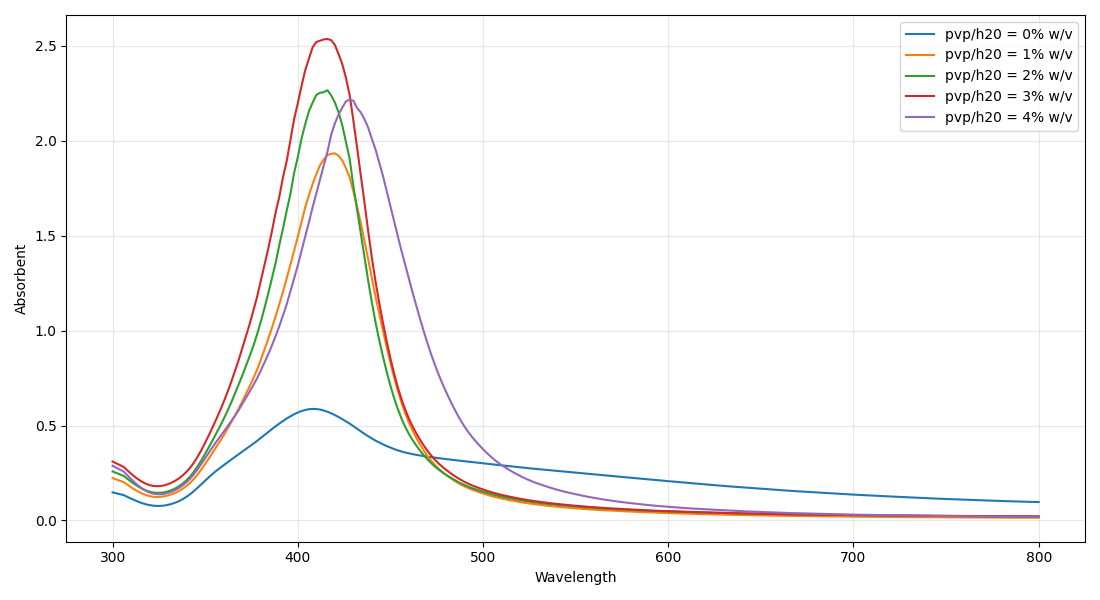
\includegraphics[width=0.95\textwidth]{figures/pvp.png}
  \caption{Phổ UV--Vis của hệ Ag@PVP tại các nồng độ PVP 0; 1; 2; 3 và 4\% (w/v).}
  \label{fig:pvp-concentration}
\end{figure}

\section{Kết quả khảo sát OFAT đối với hệ Ag@CMC}
Kết quả khảo sát đơn yếu tố đối với hệ Ag@CMC được trình bày theo trình tự tỷ lệ glycerol, nồng độ NaOH, nhiệt độ phản ứng, thời gian phản ứng và nồng độ CMC.
Đối với từng khảo sát, các yếu tố không được thay đổi được giữ cố định theo điều kiện đã lựa chọn ở bước khảo sát trước đó.
Phổ UV--Vis được sử dụng để theo dõi sự xuất hiện, vị trí và cường độ của dải hấp thụ SPR.

\subsection{Khảo sát ảnh hưởng của tỷ lệ glycerol}
Hình~\ref{fig:cmc-glycerol} trình bày phổ UV--Vis của hệ Ag@CMC khi tỷ lệ glycerol được khảo sát tại 30, 40, 50, 60 và 70\% (v/v).
Sự thay đổi vị trí, cường độ và độ rộng của dải SPR được sử dụng để đánh giá ảnh hưởng của tỷ lệ glycerol đến quá trình hình thành AgNPs.

\begin{figure}[htbp]
  \centering
  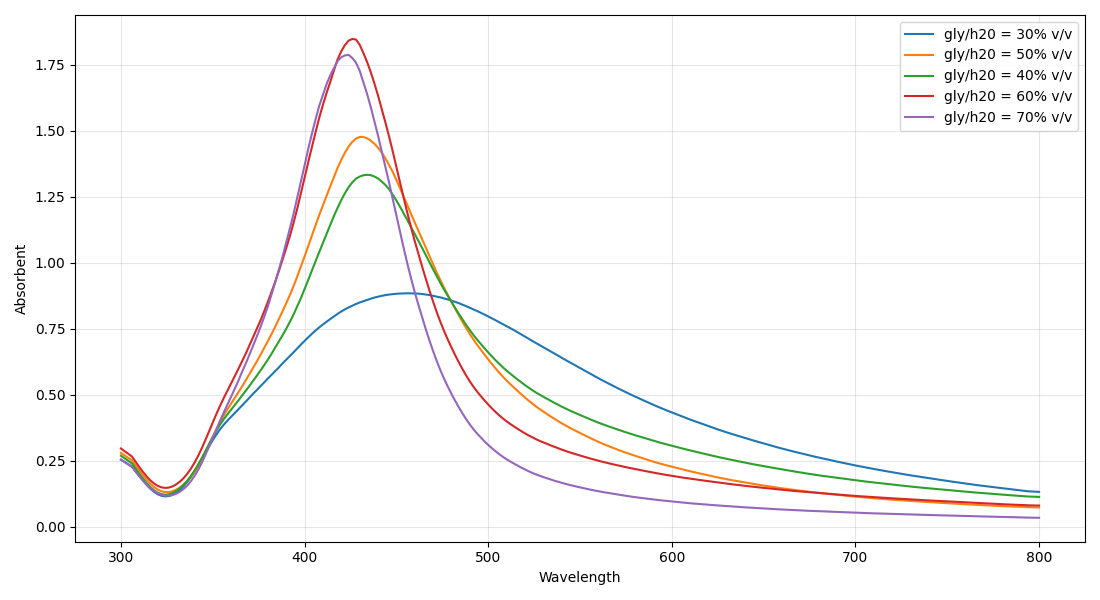
\includegraphics[width=0.95\textwidth]{figures/cmc_gly.png}
  \caption{Phổ UV--Vis của hệ Ag@CMC tại các tỷ lệ glycerol 30, 40, 50, 60 và 70\% (v/v).}
  \label{fig:cmc-glycerol}
\end{figure}

\subsection{Khảo sát ảnh hưởng của nồng độ NaOH}
Hình~\ref{fig:cmc-naoh} trình bày phổ UV--Vis của hệ Ag@CMC tại các nồng độ NaOH 1, 2, 3 và 4 mM.
Kết quả được sử dụng để đánh giá vai trò của điều kiện kiềm đối với sự hình thành và đặc trưng quang học của AgNPs.

\begin{figure}[htbp]
  \centering
  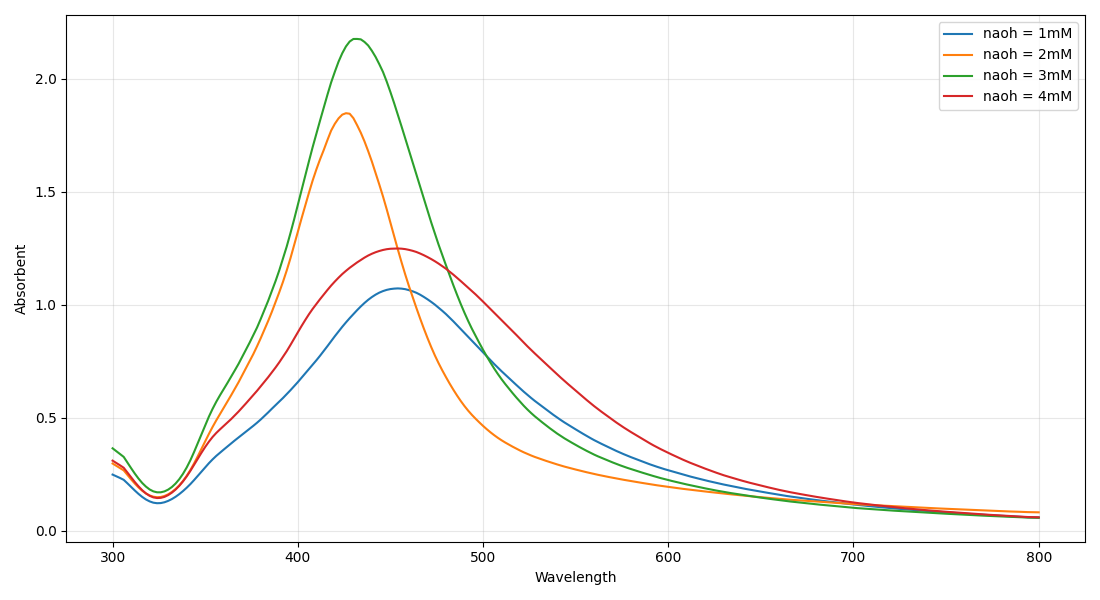
\includegraphics[width=0.95\textwidth]{figures/cmc_naoh.png}
  \caption{Phổ UV--Vis của hệ Ag@CMC tại các nồng độ NaOH 1, 2, 3 và 4 mM.}
  \label{fig:cmc-naoh}
\end{figure}

\subsection{Khảo sát ảnh hưởng của nhiệt độ phản ứng}
Hình~\ref{fig:cmc-temperature} trình bày phổ UV--Vis của hệ Ag@CMC khi nhiệt độ phản ứng được khảo sát tại 40, 50, 60, 70 và 80~$^\circ$C.
Sự thay đổi dải SPR theo nhiệt độ được xem xét cùng với các tiêu chí lựa chọn điều kiện phù hợp của hệ.

\begin{figure}[htbp]
  \centering
  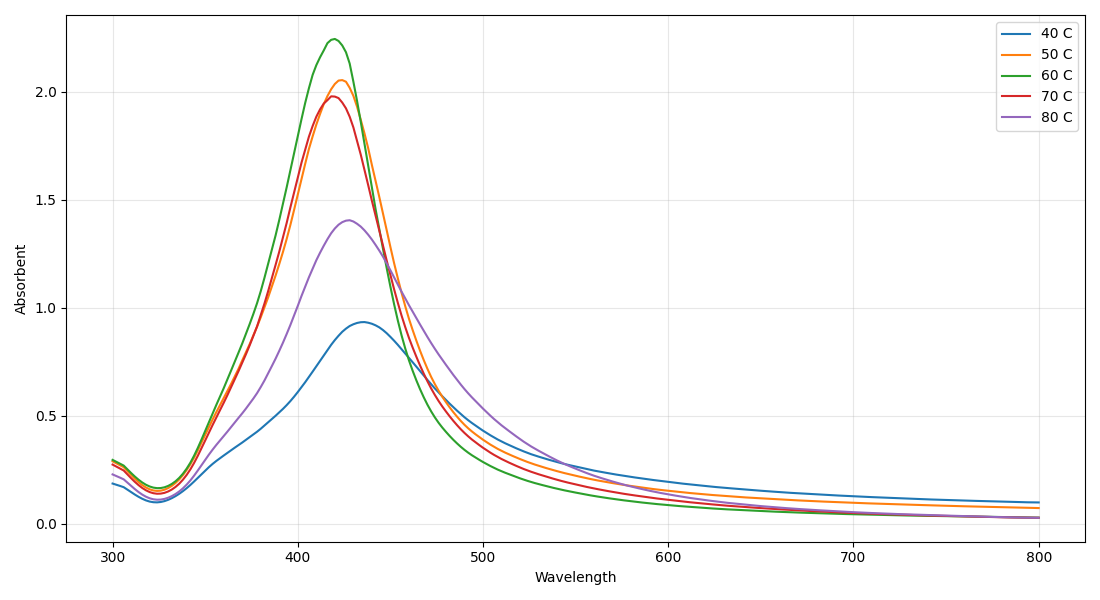
\includegraphics[width=0.95\textwidth]{figures/cmc_temp.png}
  \caption{Phổ UV--Vis của hệ Ag@CMC tại các nhiệt độ phản ứng 40, 50, 60, 70 và 80~$^\circ$C.}
  \label{fig:cmc-temperature}
\end{figure}

\subsection{Khảo sát ảnh hưởng của thời gian phản ứng}
Hình~\ref{fig:cmc-time} trình bày phổ UV--Vis của hệ Ag@CMC tại các thời điểm 5, 10, 15, 20, 25 và 30 phút.
Các phổ được sử dụng để theo dõi diễn biến hình thành AgNPs theo thời gian phản ứng.

\begin{figure}[htbp]
  \centering
  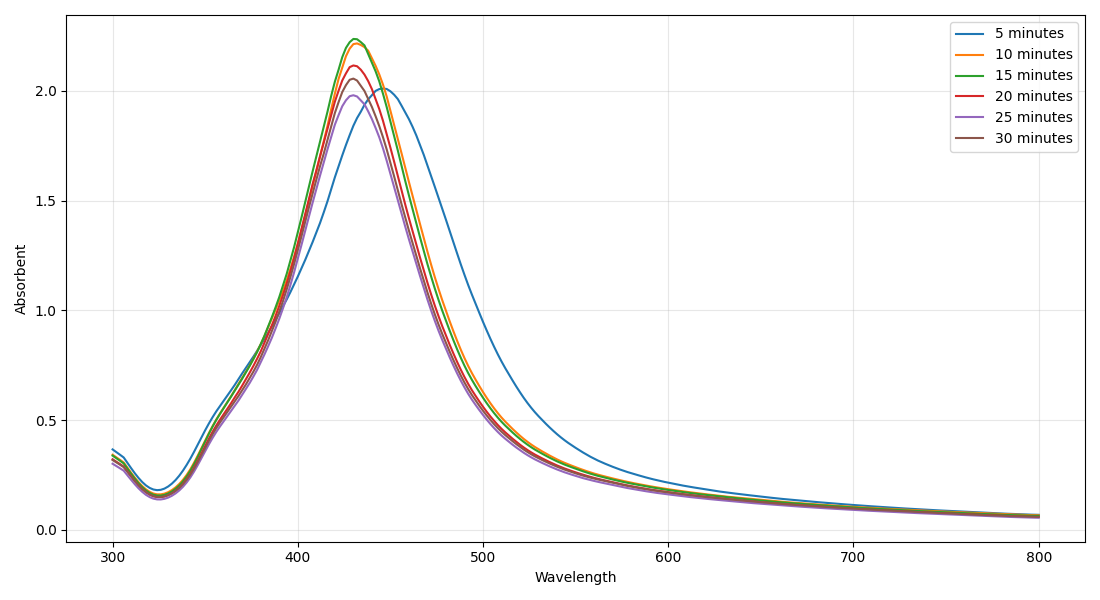
\includegraphics[width=0.95\textwidth]{figures/cmc_time.png}
  \caption{Phổ UV--Vis của hệ Ag@CMC tại các thời gian phản ứng 5, 10, 15, 20, 25 và 30 phút.}
  \label{fig:cmc-time}
\end{figure}

\subsection{Khảo sát ảnh hưởng của nồng độ CMC}
Hình~\ref{fig:cmc-concentration} trình bày phổ UV--Vis của hệ Ag@CMC khi nồng độ CMC được khảo sát tại 0,3; 0,6 và 0,9\% (w/v).
Các phổ này được sử dụng để đánh giá ảnh hưởng của hàm lượng CMC đến trạng thái phân tán và đáp ứng quang học của AgNPs.

\begin{figure}[htbp]
  \centering
  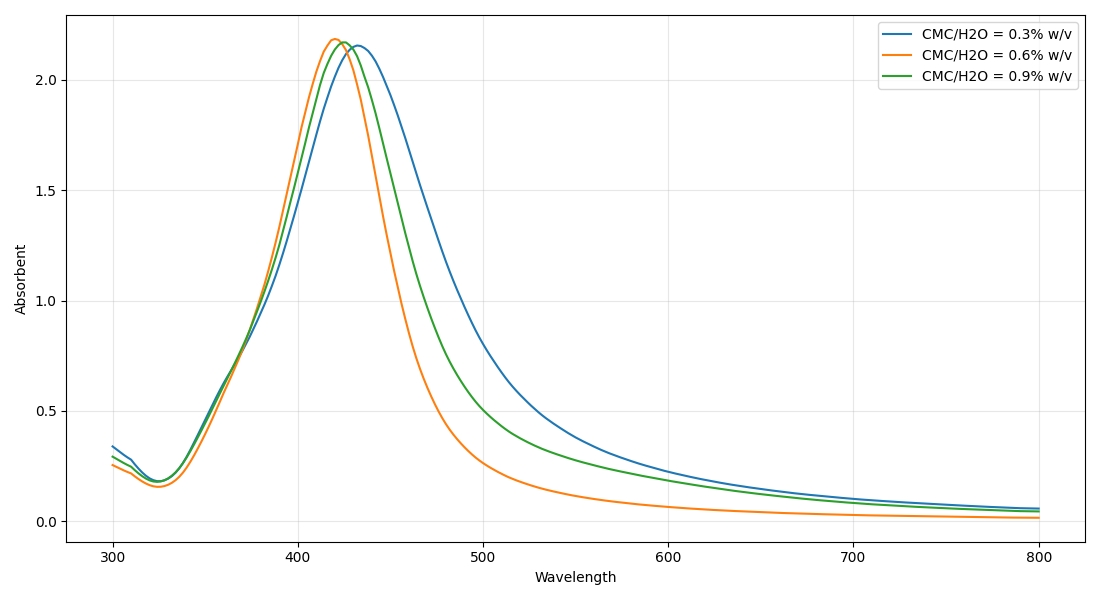
\includegraphics[width=0.95\textwidth]{figures/cmc.png}
  \caption{Phổ UV--Vis của hệ Ag@CMC tại các nồng độ CMC 0,3; 0,6 và 0,9\% (w/v).}
  \label{fig:cmc-concentration}
\end{figure}

\section{Đặc trưng AgNPs tại điều kiện tối ưu}
\subsection{Kích thước, phân bố kích thước và điện thế zeta}
Trình bày kết quả DLS và điện thế zeta của mẫu tối ưu; đối chiếu với tiêu chí đã đặt ra.

\subsection{Hình thái và cấu trúc vật liệu}
Trình bày ảnh TEM/SEM, giản đồ XRD và phổ FTIR của mẫu tối ưu. Thảo luận kích thước thực, hình dạng, pha tinh thể và tương tác bề mặt.

\section{So sánh hiệu quả bảo vệ hạt của PVP và CMC}
\subsection{Ảnh hưởng đến quá trình hình thành AgNPs}
So sánh màu sắc, phổ UV-Vis và tốc độ hình thành hạt ở hai hệ PVP và CMC trong cùng điều kiện phản ứng.

\subsection{Ảnh hưởng đến kích thước và hình thái hạt}
So sánh kết quả DLS, TEM/SEM và chỉ số đa phân tán để đánh giá khả năng kiểm soát kích thước của mỗi capping agent.

\subsection{Đánh giá độ ổn định theo thời gian}
Theo dõi sự thay đổi phổ UV-Vis, kích thước và điện thế zeta trong thời gian bảo quản đã lựa chọn.

\subsection{Đánh giá độ ổn định theo pH, nhiệt độ và lực ion}
So sánh độ bền của hai hệ khi thay đổi pH, nhiệt độ hoặc nồng độ muối điện ly. Xác định điều kiện gây kết tụ hoặc mất ổn định rõ rệt.

\subsection{Thảo luận cơ chế bảo vệ}
Diễn giải kết quả dựa trên cơ chế cản trở không gian của PVP và cơ chế ổn định điện tích của CMC. Liên hệ điện thế zeta, dữ liệu FTIR và khả năng chống kết tụ để rút ra nhận định.

\section{Tổng hợp kết quả thảo luận}
Tóm tắt các thông số tối ưu, đặc trưng AgNPs thu được và chất bảo vệ phù hợp theo từng tiêu chí đánh giá.
